\documentclass[11pt, letterpaper]{article}

% Fonts and Encoding
\usepackage[utf8]{inputenc}
\usepackage[T1]{fontenc}
\usepackage{lmodern} % High-quality Latin Modern vector font

% Math and Symbols
\usepackage{amsmath, amssymb, amsthm, amsfonts, mathrsfs, mathtools}

% Layout and Geometry
\usepackage{geometry}
\geometry{letterpaper, margin=1in}
\setlength{\parindent}{0pt}
\setlength{\parskip}{0.6em}

% Formatting and Graphics
\usepackage{graphicx, xcolor, enumitem, booktabs, array, tabularx}

% TikZ for Illustrations
\usepackage{tikz}
\usetikzlibrary{arrows.meta, positioning, shapes.geometric, calc, backgrounds, matrix}

% Clickable Links and TOC
\usepackage{hyperref}
\hypersetup{
    colorlinks=true,
    linkcolor=blue,
    filecolor=magenta,      
    urlcolor=cyan,
    pdftitle={Mastering Quadratic Forms},
}

% Theorem Environments
\newtheorem{theorem}{Theorem}[section]
\newtheorem{lemma}[theorem]{Lemma}
\newtheorem{proposition}[theorem]{Proposition}
\newtheorem{corollary}[theorem]{Corollary}
\theoremstyle{definition}
\newtheorem{definition}{Definition}[section]
\newtheorem{axiom}{Axiom}[section]
\newtheorem{example}{Example}[section]
\theoremstyle{remark}
\newtheorem{remark}{Remark}[section]

% Custom Commands (Enforced standard notation)
\newcommand{\R}{\mathbb{R}}
\newcommand{\N}{\mathbb{N}}
\newcommand{\Z}{\mathbb{Z}}
\newcommand{\Q}{\mathbb{Q}}
\newcommand{\E}{\mathbb{E}}
\newcommand{\Prob}{\mathbb{P}}
\newcommand{\F}{\mathcal{F}}
\newcommand{\x}{\mathbf{x}}
\newcommand{\y}{\mathbf{y}}

\title{\Huge \textbf{Mastering Quadratic Forms} \\ \Large A Comprehensive Guide and Solution Manual}
\author{Tashfeen Omran}
\date{}

\begin{document}

\maketitle
\tableofcontents
\newpage

% ==========================================
% PART 1: INTRODUCTION
% ==========================================
\section{Part 1: Comprehensive Introduction, Context, and Prerequisites}

\subsection{Core Concepts}
A \textbf{quadratic form} on $\R^n$ is a function $Q$ defined on $\R^n$ whose value at a vector $\x$ can be computed by an expression of the form:
\[
Q(\x) = \x^T A \x
\]
where $A$ is an $n \times n$ \textbf{symmetric matrix} ($A = A^T$). The matrix $A$ is called the \textit{matrix of the quadratic form}. 

When you expand the matrix multiplication $\x^T A \x$, you obtain a polynomial where every term has a degree of exactly two (e.g., $x_1^2$, $x_2^2$, or cross-products like $x_1 x_2$). The diagonal entries of $A$ correspond to the coefficients of the squared terms ($x_i^2$), while the off-diagonal entries $A_{ij}$ and $A_{ji}$ evenly split the coefficient of the cross-product term $x_i x_j$.

\subsection{Intuition and Derivation}
Geometrically, setting a quadratic form equal to a constant, $Q(\x) = c$, defines a conic section (in $\R^2$) or a quadric surface (in $\R^3$). If the matrix $A$ is diagonal, the equation has no cross-product terms, meaning the geometric shape is in \textit{standard position} (its axes of symmetry align with the coordinate axes). 

When cross-product terms are present, the shape is rotated. The \textbf{Principal Axes Theorem} states that we can always eliminate these cross-product terms by rotating our coordinate system. We do this by finding an orthogonal matrix $P$ whose columns are the eigenvectors of $A$. By making the substitution $\x = P\y$, the quadratic form simplifies to:
\[
\x^T A \x = (P\y)^T A (P\y) = \y^T (P^T A P) \y = \y^T D \y = \lambda_1 y_1^2 + \lambda_2 y_2^2 + \dots + \lambda_n y_n^2
\]
where $D$ is a diagonal matrix containing the eigenvalues of $A$.

\begin{center}
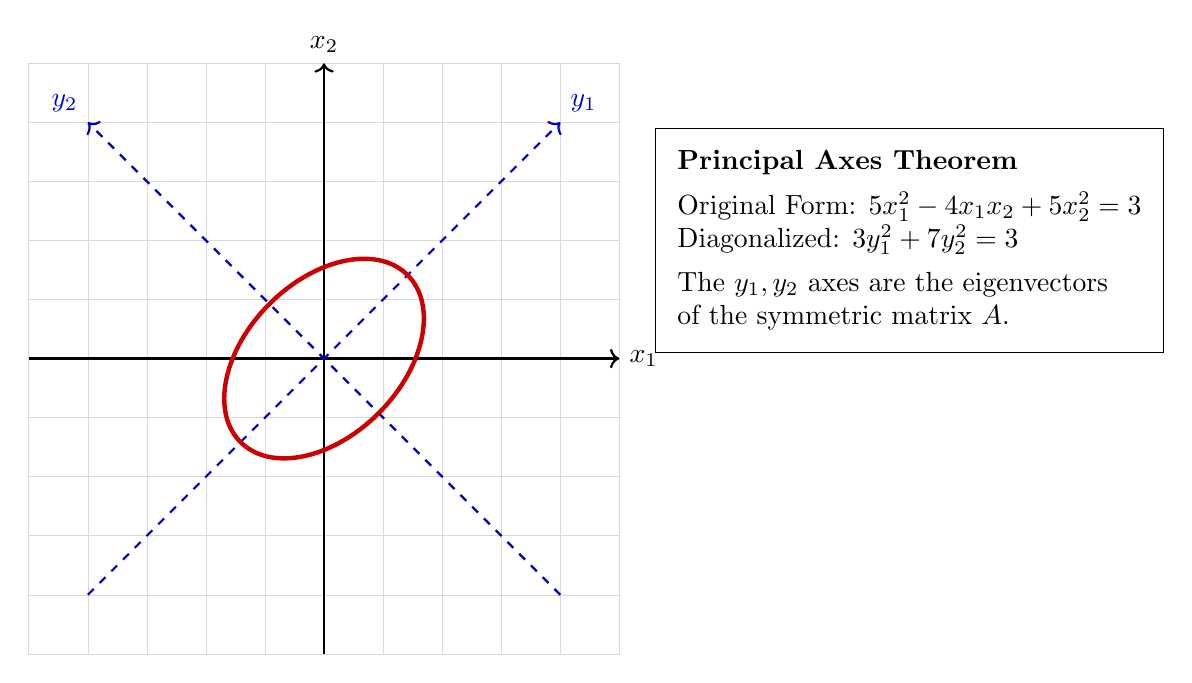
\begin{tikzpicture}[scale=1.5]
    % Background/Grid
    \draw[step=0.5, gray!30, very thin] (-2.5,-2.5) grid (2.5,2.5);
    
    % Axes
    \draw[->, thick] (-2.5,0) -- (2.5,0) node[right] {$x_1$};
    \draw[->, thick] (0,-2.5) -- (0,2.5) node[above] {$x_2$};
    
    % Principal Axes (rotated by 45 degrees)
    \draw[->, thick, dashed, blue!80!black] (-2,-2) -- (2,2) node[above right] {$y_1$};
    \draw[->, thick, dashed, blue!80!black] (2,-2) -- (-2,2) node[above left] {$y_2$};
    
    % Ellipse: 5x_1^2 - 4x_1 x_2 + 5x_2^2 = 3
    % In y coordinates: 3y_1^2 + 7y_2^2 = 3 => y_1^2/1^2 + y_2^2/(sqrt(3/7))^2 = 1
    \draw[ultra thick, red!80!black, rotate=45] (0,0) ellipse (1cm and 0.654cm);
    
    % Legend
    \node[align=left, anchor=west, inner sep=8pt, draw, fill=white] at (2.8, 1) {
        \textbf{Principal Axes Theorem} \\[4pt]
        Original Form: $5x_1^2 - 4x_1x_2 + 5x_2^2 = 3$ \\
        Diagonalized: $3y_1^2 + 7y_2^2 = 3$ \\[4pt]
        The $y_1, y_2$ axes are the eigenvectors \\
        of the symmetric matrix $A$.
    };
\end{tikzpicture}
\end{center}

\subsection{Historical Context and Motivation}
The study of quadratic forms dates back to mathematicians like Carl Friedrich Gauss and Joseph-Louis Lagrange in the 18th and 19th centuries, who were interested in number theory (e.g., which integers can be represented as the sum of two squares). Later, in the context of geometry and physics, quadratic forms became essential for understanding kinetic and potential energy in classical mechanics, where energy is proportional to the square of velocity or position. Today, they are the bedrock of optimization, statistics (variance-covariance matrices), and machine learning.

\subsection{Key Formulas}
\renewcommand{\arraystretch}{1.5}
\begin{tabularx}{\textwidth}{>{\raggedright\arraybackslash}X >{$\displaystyle}c<{$}}
\toprule
\textbf{Concept} & \textbf{Formula} \\
\midrule
Quadratic Form Definition & Q(\x) = \x^T A \x \\
Change of Variable & \x = P\y \implies Q(P\y) = \y^T (P^T A P) \y \\
Diagonalized Form & \y^T D \y = \lambda_1 y_1^2 + \lambda_2 y_2^2 + \dots + \lambda_n y_n^2 \\
Constrained Optimization & \max_{\|\x\|=1} \x^T A \x = \lambda_{\text{max}}, \quad \min_{\|\x\|=1} \x^T A \x = \lambda_{\text{min}} \\
\bottomrule
\end{tabularx}

\subsection{Prerequisites}
To master this section, you must be comfortable with:
\begin{itemize}
    \item \textbf{Matrix Multiplication:} Computing $\x^T A \x$.
    \item \textbf{Eigenvalues and Eigenvectors:} Solving $\det(A - \lambda I) = 0$ and finding the null space of $A - \lambda I$.
    \item \textbf{Orthogonal Diagonalization:} Normalizing eigenvectors to form an orthogonal matrix $P$ such that $P^T P = I$ and $P^T A P = D$.
\end{itemize}

\newpage

% ==========================================
% PART 2: HOMEWORK SOLUTIONS
% ==========================================
\section{Part 2: Detailed Homework Solutions}

\subsection{Exercises 1--6: Computing and Finding Matrices}

\textbf{Problem 1:} Compute the quadratic form $\x^T A \x$, when $A = \begin{bmatrix} 3 & 1/4 \\ 1/4 & 1 \end{bmatrix}$ and 
a. $\x = \begin{bmatrix} x_1 \\ x_2 \end{bmatrix}$, b. $\x = \begin{bmatrix} 8 \\ 1 \end{bmatrix}$, c. $\x = \begin{bmatrix} 1 \\ 4 \end{bmatrix}$.

\textit{Solution:}
\begin{itemize}
    \item[\textbf{a.}] $\x^T A \x = 3x_1^2 + \left(\frac{1}{4} + \frac{1}{4}\right)x_1 x_2 + 1x_2^2 = 3x_1^2 + \frac{1}{2}x_1 x_2 + x_2^2$.
    \item[\textbf{b.}] Substitute $x_1 = 8, x_2 = 1$: $3(8)^2 + \frac{1}{2}(8)(1) + (1)^2 = 3(64) + 4 + 1 = 192 + 4 + 1 = 197$.
    \item[\textbf{c.}] Substitute $x_1 = 1, x_2 = 4$: $3(1)^2 + \frac{1}{2}(1)(4) + (4)^2 = 3 + 2 + 16 = 21$.
\end{itemize}

\textbf{Problem 2:} Compute $\x^T A \x$, for $A = \begin{bmatrix} 4 & 1 & 0 \\ 1 & 1 & 3 \\ 0 & 3 & 0 \end{bmatrix}$ and 
a. $\x = \begin{bmatrix} x_1 \\ x_2 \\ x_3 \end{bmatrix}$, b. $\x = \begin{bmatrix} -3 \\ -1 \\ 4 \end{bmatrix}$, c. $\x = \begin{bmatrix} 1/\sqrt{5} \\ 1/\sqrt{5} \\ 1/\sqrt{5} \end{bmatrix}$.

\textit{Solution:}
\begin{itemize}
    \item[\textbf{a.}] $\x^T A \x = 4x_1^2 + 1x_2^2 + 0x_3^2 + (1+1)x_1 x_2 + (0+0)x_1 x_3 + (3+3)x_2 x_3 = 4x_1^2 + x_2^2 + 2x_1 x_2 + 6x_2 x_3$.
    \item[\textbf{b.}] Substitute $x_1 = -3, x_2 = -1, x_3 = 4$: $4(-3)^2 + (-1)^2 + 2(-3)(-1) + 6(-1)(4) = 36 + 1 + 6 - 24 = 19$.
    \item[\textbf{c.}] Substitute $x_1 = x_2 = x_3 = 1/\sqrt{5}$: $4(1/5) + 1/5 + 2(1/5) + 6(1/5) = \frac{13}{5}$.
\end{itemize}

\textbf{Problem 3:} Find the matrix of the quadratic form. Assume $\x$ is in $\R^2$.
a. $4x_1^2 - 6x_1 x_2 + 5x_2^2 \quad$ b. $5x_1^2 + 4x_1 x_2$

\textit{Solution:} The diagonal entries are the coefficients of the squared terms. The off-diagonal entries are half the cross-product coefficients.
\begin{itemize}
    \item[\textbf{a.}] $A_{11} = 4, A_{22} = 5, A_{12} = A_{21} = -6/2 = -3 \implies A = \begin{bmatrix} 4 & -3 \\ -3 & 5 \end{bmatrix}$.
    \item[\textbf{b.}] $A_{11} = 5, A_{22} = 0, A_{12} = A_{21} = 4/2 = 2 \implies A = \begin{bmatrix} 5 & 2 \\ 2 & 0 \end{bmatrix}$.
\end{itemize}

\textbf{Problem 4:} Find the matrix of the quadratic form. Assume $\x$ is in $\R^2$.
a. $7x_1^2 + 18x_1 x_2 - 7x_2^2 \quad$ b. $8x_1 x_2$

\textit{Solution:}
\begin{itemize}
    \item[\textbf{a.}] $A = \begin{bmatrix} 7 & 9 \\ 9 & -7 \end{bmatrix}$.
    \item[\textbf{b.}] $A = \begin{bmatrix} 0 & 4 \\ 4 & 0 \end{bmatrix}$.
\end{itemize}

\textbf{Problem 5:} Find the matrix of the quadratic form. Assume $\x$ is in $\R^3$.
a. $5x_1^2 + 3x_2^2 - 7x_3^2 - 4x_1 x_2 + 6x_1 x_3 - 2x_2 x_3 \quad$ b. $8x_1 x_2 + 10x_1 x_3 - 6x_2 x_3$

\textit{Solution:}
\begin{itemize}
    \item[\textbf{a.}] $A = \begin{bmatrix} 5 & -2 & 3 \\ -2 & 3 & -1 \\ 3 & -1 & -7 \end{bmatrix}$.
    \item[\textbf{b.}] $A = \begin{bmatrix} 0 & 4 & 5 \\ 4 & 0 & -3 \\ 5 & -3 & 0 \end{bmatrix}$.
\end{itemize}

\textbf{Problem 6:} Find the matrix of the quadratic form. Assume $\x$ is in $\R^3$.
a. $5x_1^2 - 3x_2^2 + 7x_3^2 + 8x_1 x_2 - 4x_1 x_3 \quad$ b. $6x_3^2 - 4x_1 x_2 - 2x_2 x_3$

\textit{Solution:}
\begin{itemize}
    \item[\textbf{a.}] $A = \begin{bmatrix} 5 & 4 & -2 \\ 4 & -3 & 0 \\ -2 & 0 & 7 \end{bmatrix}$.
    \item[\textbf{b.}] $A = \begin{bmatrix} 0 & -2 & 0 \\ -2 & 0 & -1 \\ 0 & -1 & 6 \end{bmatrix}$.
\end{itemize}

\subsection{Exercises 7--18: Change of Variable and Classification}

\textbf{Problem 7:} Make the change of variable, $\x = P\y$, that transforms $x_1^2 + 12x_1 x_2 + x_2^2$ into a quadratic form with no cross-product terms. Give $P$ and the new quadratic form.

\textit{Solution:}
The matrix is $A = \begin{bmatrix} 1 & 6 \\ 6 & 1 \end{bmatrix}$. 
Characteristic equation: $\det(A - \lambda I) = (1-\lambda)^2 - 36 = \lambda^2 - 2\lambda - 35 = (\lambda - 7)(\lambda + 5) = 0$.
Eigenvalues are $\lambda_1 = 7, \lambda_2 = -5$.
For $\lambda_1 = 7$: $A - 7I = \begin{bmatrix} -6 & 6 \\ 6 & -6 \end{bmatrix} \implies$ eigenvector $\mathbf{v}_1 = \begin{bmatrix} 1 \\ 1 \end{bmatrix}$. Normalized: $\mathbf{u}_1 = \begin{bmatrix} 1/\sqrt{2} \\ 1/\sqrt{2} \end{bmatrix}$.
For $\lambda_2 = -5$: $A + 5I = \begin{bmatrix} 6 & 6 \\ 6 & 6 \end{bmatrix} \implies$ eigenvector $\mathbf{v}_2 = \begin{bmatrix} -1 \\ 1 \end{bmatrix}$. Normalized: $\mathbf{u}_2 = \begin{bmatrix} -1/\sqrt{2} \\ 1/\sqrt{2} \end{bmatrix}$.
Thus, $P = \begin{bmatrix} 1/\sqrt{2} & -1/\sqrt{2} \\ 1/\sqrt{2} & 1/\sqrt{2} \end{bmatrix}$. The new quadratic form is $\y^T D \y = 7y_1^2 - 5y_2^2$.

\textbf{Problem 8:} Let $A$ be the matrix of $7x_1^2 + 5x_2^2 + 9x_3^2 - 8x_1 x_2 + 8x_1 x_3$. Eigenvalues are 1, 7, 13. Find $P$ and the new quadratic form.

\textit{Solution:}
$A = \begin{bmatrix} 7 & -4 & 4 \\ -4 & 5 & 0 \\ 4 & 0 & 9 \end{bmatrix}$.
For $\lambda = 1$: $A - I = \begin{bmatrix} 6 & -4 & 4 \\ -4 & 4 & 0 \\ 4 & 0 & 8 \end{bmatrix} \implies \mathbf{v}_1 = \begin{bmatrix} 2 \\ 2 \\ -1 \end{bmatrix}$.
For $\lambda = 7$: $A - 7I = \begin{bmatrix} 0 & -4 & 4 \\ -4 & -2 & 0 \\ 4 & 0 & 2 \end{bmatrix} \implies \mathbf{v}_2 = \begin{bmatrix} -1 \\ 2 \\ 2 \end{bmatrix}$.
For $\lambda = 13$: $A - 13I = \begin{bmatrix} -6 & -4 & 4 \\ -4 & -8 & 0 \\ 4 & 0 & -4 \end{bmatrix} \implies \mathbf{v}_3 = \begin{bmatrix} 2 \\ -1 \\ 2 \end{bmatrix}$.
Normalizing these vectors (each has length $\sqrt{4+4+1} = 3$), we get:
$P = \frac{1}{3} \begin{bmatrix} 2 & -1 & 2 \\ 2 & 2 & -1 \\ -1 & 2 & 2 \end{bmatrix}$. The new form is $y_1^2 + 7y_2^2 + 13y_3^2$.

\textbf{Problems 9--14:} Classify the quadratic forms, find $P$, and write the new form.
\begin{itemize}
    \item[\textbf{9.}] $6x_1^2 - 4x_1 x_2 + 3x_2^2 \implies A = \begin{bmatrix} 6 & -2 \\ -2 & 3 \end{bmatrix}$. Eigenvalues: $\lambda = 2, 7$. \textbf{Positive definite}. \\
    $P = \frac{1}{\sqrt{5}} \begin{bmatrix} 1 & -2 \\ 2 & 1 \end{bmatrix}$. New form: $2y_1^2 + 7y_2^2$.
    
    \item[\textbf{10.}] $3x_1^2 + 8x_1 x_2 - 3x_2^2 \implies A = \begin{bmatrix} 3 & 4 \\ 4 & -3 \end{bmatrix}$. Eigenvalues: $\lambda = 5, -5$. \textbf{Indefinite}. \\
    $P = \frac{1}{\sqrt{5}} \begin{bmatrix} 2 & -1 \\ 1 & 2 \end{bmatrix}$. New form: $5y_1^2 - 5y_2^2$.
    
    \item[\textbf{11.}] $4x_1^2 - 8x_1 x_2 - 2x_2^2 \implies A = \begin{bmatrix} 4 & -4 \\ -4 & -2 \end{bmatrix}$. Eigenvalues: $\lambda = 6, -4$. \textbf{Indefinite}. \\
    $P = \frac{1}{\sqrt{5}} \begin{bmatrix} -2 & 1 \\ 1 & 2 \end{bmatrix}$. New form: $6y_1^2 - 4y_2^2$.
    
    \item[\textbf{12.}] $-2x_1^2 - 4x_1 x_2 - 2x_2^2 \implies A = \begin{bmatrix} -2 & -2 \\ -2 & -2 \end{bmatrix}$. Eigenvalues: $\lambda = 0, -4$. \textbf{Negative semidefinite}. \\
    $P = \frac{1}{\sqrt{2}} \begin{bmatrix} -1 & 1 \\ 1 & 1 \end{bmatrix}$. New form: $-4y_2^2$.
    
    \item[\textbf{13.}] $x_1^2 - 4x_1 x_2 + 4x_2^2 \implies A = \begin{bmatrix} 1 & -2 \\ -2 & 4 \end{bmatrix}$. Eigenvalues: $\lambda = 0, 5$. \textbf{Positive semidefinite}. \\
    $P = \frac{1}{\sqrt{5}} \begin{bmatrix} 2 & -1 \\ 1 & 2 \end{bmatrix}$. New form: $5y_2^2$.
    
    \item[\textbf{14.}] $5x_1^2 + 12x_1 x_2 \implies A = \begin{bmatrix} 5 & 6 \\ 6 & 0 \end{bmatrix}$. Eigenvalues: $\lambda = 9, -4$. \textbf{Indefinite}. \\
    $P = \frac{1}{\sqrt{13}} \begin{bmatrix} 3 & -2 \\ 2 & 3 \end{bmatrix}$. New form: $9y_1^2 - 4y_2^2$.
\end{itemize}

\textbf{Problems 15--18 (Advanced $4 \times 4$ Matrices):}
\begin{itemize}
    \item[\textbf{15.}] $A = \begin{bmatrix} -3 & 2 & 2 & 2 \\ 2 & -7 & 0 & 0 \\ 2 & 0 & -10 & 3 \\ 2 & 0 & 3 & -10 \end{bmatrix}$. By inspection, $\mathbf{v}_1 = (0, -2, 1, 1)^T$ yields $A\mathbf{v}_1 = -7\mathbf{v}_1$, and $\mathbf{v}_2 = (0, 0, 1, -1)^T$ yields $A\mathbf{v}_2 = -13\mathbf{v}_2$. The remaining orthogonal eigenvectors take the form $(a, c, c, c)^T$, yielding $\lambda = -1, -9$ with eigenvectors $(3, 1, 1, 1)^T$ and $(-1, 1, 1, 1)^T$. All eigenvalues ($-1, -7, -9, -13$) are negative. \textbf{Negative definite}. \\
    $P = \begin{bmatrix} 0 & 0 & 3/\sqrt{12} & -1/2 \\ -2/\sqrt{6} & 0 & 1/\sqrt{12} & 1/2 \\ 1/\sqrt{6} & 1/\sqrt{2} & 1/\sqrt{12} & 1/2 \\ 1/\sqrt{6} & -1/\sqrt{2} & 1/\sqrt{12} & 1/2 \end{bmatrix}$. New form: $-y_1^2 - 7y_2^2 - 9y_3^2 - 13y_4^2$.

    \item[\textbf{16.}] $A = \begin{bmatrix} 4 & 4 & 0 & -3 \\ 4 & 4 & 3 & 0 \\ 0 & 3 & 4 & 4 \\ -3 & 0 & 4 & 4 \end{bmatrix}$. Using symmetry, eigenvectors of the form $(a, b, b, a)^T$ and $(c, d, -d, -c)^T$ yield eigenvalues $9, 9, -1, -1$. \textbf{Indefinite}. \\
    $P = \frac{1}{\sqrt{10}} \begin{bmatrix} 1 & 2 & 2 & 1 \\ 2 & 1 & -1 & -2 \\ 2 & -1 & -1 & 2 \\ 1 & -2 & 2 & -1 \end{bmatrix}$. New form: $9y_1^2 + 9y_2^2 - y_3^2 - y_4^2$.

    \item[\textbf{17.}] $A = \begin{bmatrix} 11 & 8 & 0 & -6 \\ 8 & 11 & 6 & 0 \\ 0 & 6 & 11 & 8 \\ -6 & 0 & 8 & 11 \end{bmatrix}$. Using the exact same eigenvectors as Problem 16, the eigenvalues are $21, 21, 1, 1$. \textbf{Positive definite}. \\
    $P$ is identical to Problem 16. New form: $21y_1^2 + 21y_2^2 + y_3^2 + y_4^2$.

    \item[\textbf{18.}] $A = \begin{bmatrix} 2 & -3 & -3 & -3 \\ -3 & 2 & -3 & -3 \\ -3 & -3 & 0 & -1 \\ -3 & -3 & -1 & 0 \end{bmatrix}$. Eigenvalues are $5, 5, 1, -7$. \textbf{Indefinite}. \\
    $P = \begin{bmatrix} 1/\sqrt{2} & 1/2 & 0 & 1/2 \\ -1/\sqrt{2} & 1/2 & 0 & 1/2 \\ 0 & -1/2 & 1/\sqrt{2} & 1/2 \\ 0 & -1/2 & -1/\sqrt{2} & 1/2 \end{bmatrix}$. New form: $5y_1^2 + 5y_2^2 + y_3^2 - 7y_4^2$.
\end{itemize}

\subsection{Exercises 19--20: Constrained Optimization}

\textbf{Problem 19:} What is the largest possible value of $4x_1^2 + 9x_2^2$ if $\x^T \x = 1$? \\
\textit{Solution:} The matrix is diagonal with eigenvalues 4 and 9. The maximum value on the unit sphere is the largest eigenvalue, which is \textbf{9}.

\textbf{Problem 20:} What is the largest possible value of $7x_1^2 - 5x_2^2$ if $\x^T \x = 1$? \\
\textit{Solution:} The eigenvalues are 7 and -5. The maximum value is \textbf{7}.

\subsection{Exercises 21--30: True/False Questions}
\begin{enumerate}[label=\textbf{\arabic*.}, start=21]
    \item \textbf{True.} By definition, the matrix $A$ in $Q(\x) = \x^T A \x$ is constructed to be symmetric.
    \item \textbf{False.} $\|\x\|^2 = x_1^2 + \dots + x_n^2 = \x^T I \x$, which is a quadratic form with matrix $I$.
    \item \textbf{True.} If $A$ is diagonal, $A_{ij} = 0$ for $i \neq j$, meaning all cross-product coefficients are zero.
    \item \textbf{False.} $P$ must specifically be the orthogonal matrix whose columns are the eigenvectors of $A$. An arbitrary orthogonal matrix will not necessarily diagonalize $A$.
    \item \textbf{True.} The principal axes are defined by the columns of the diagonalizing matrix $P$, which are the eigenvectors of $A$.
    \item \textbf{True.} By Theorem 5, a quadratic form is positive definite if and only if all eigenvalues of $A$ are positive.
    \item \textbf{False.} A positive definite form satisfies $Q(\x) > 0$ for all $\x \neq \mathbf{0}$. At $\x = \mathbf{0}$, $Q(\mathbf{0}) = 0$.
    \item \textbf{True.} An indefinite form takes both positive and negative values, so it cannot be $\ge 0$ everywhere (positive semidefinite) or $\le 0$ everywhere (negative semidefinite).
    \item \textbf{True.} A Cholesky factorization $A = R^T R$ with positive diagonal entries exists if and only if $A$ is positive definite.
    \item \textbf{False.} If $Q(\x) < 0$ for all $\x \neq \mathbf{0}$, the form is negative definite, meaning all eigenvalues are negative, not positive.
\end{enumerate}

\subsection{Exercises 31--36: Theoretical Proofs}

\textbf{Problem 31:} Show $\lambda_1 + \lambda_2 = a+d$ and $\lambda_1 \lambda_2 = \det A$. \\
\textit{Proof:} Let $A = \begin{bmatrix} a & b \\ b & d \end{bmatrix}$. The characteristic polynomial is $\det(A - \lambda I) = (a-\lambda)(d-\lambda) - b^2 = \lambda^2 - (a+d)\lambda + (ad-b^2)$. Since the roots are $\lambda_1, \lambda_2$, the polynomial factors as $(\lambda - \lambda_1)(\lambda - \lambda_2) = \lambda^2 - (\lambda_1 + \lambda_2)\lambda + \lambda_1 \lambda_2$. Equating coefficients yields $\lambda_1 + \lambda_2 = a+d$ and $\lambda_1 \lambda_2 = ad-b^2 = \det A$. \qed

\textbf{Problem 32:} Verify statements about $Q$ using $\det A$ and $a$. \\
\textit{Proof:} 
a. If $\det A > 0$, then $\lambda_1 \lambda_2 > 0$, so the eigenvalues share the same sign. Since $ad - b^2 > 0$ and $a > 0$, we must have $d > 0$. Thus $\lambda_1 + \lambda_2 = a+d > 0$. Since they share the same sign and sum to a positive number, both are positive. $Q$ is positive definite. \\
b. If $\det A > 0$ and $a < 0$, then $d < 0$. Thus $\lambda_1 + \lambda_2 = a+d < 0$. Both eigenvalues are negative. $Q$ is negative definite. \\
c. If $\det A < 0$, then $\lambda_1 \lambda_2 < 0$, meaning the eigenvalues have opposite signs. $Q$ is indefinite. \qed

\textbf{Problem 33:} Show $B^T B$ is positive semidefinite; if invertible, positive definite. \\
\textit{Proof:} For any $\x$, $\x^T (B^T B) \x = (B\x)^T (B\x) = \|B\x\|^2 \ge 0$. Thus $B^T B$ is positive semidefinite. If $B$ is invertible, $B\x = \mathbf{0} \iff \x = \mathbf{0}$. Thus for $\x \neq \mathbf{0}$, $\|B\x\|^2 > 0$, making it positive definite. \qed

\textbf{Problem 34:} Show if $A$ is positive definite, there exists positive definite $B$ such that $A = B^T B$. \\
\textit{Proof:} Since $A$ is positive definite, it can be orthogonally diagonalized as $A = P D P^T$, where $D$ has positive diagonal entries. Let $C$ be the diagonal matrix whose entries are the square roots of the entries of $D$. Then $C^T C = C^2 = D$. Let $B = P C P^T$. Then $B^T B = (P C P^T)^T (P C P^T) = P C^T P^T P C P^T = P C^2 P^T = P D P^T = A$. Since $C$ has positive diagonal entries, $B$ has positive eigenvalues and is positive definite. \qed

\textbf{Problem 35:} Show eigenvalues of $A+B$ are positive if $A, B$ are positive definite. \\
\textit{Proof:} Let $\x \neq \mathbf{0}$. Since $A$ and $B$ are positive definite, $\x^T A \x > 0$ and $\x^T B \x > 0$. Then $\x^T (A+B) \x = \x^T A \x + \x^T B \x > 0$. Thus $A+B$ is positive definite, which implies all its eigenvalues are positive. \qed

\textbf{Problem 36:} Show if $\x^T A \x$ is positive definite, so is $\x^T A^{-1} \x$. \\
\textit{Proof:} If $A$ is positive definite, its eigenvalues $\lambda_i$ are all strictly positive. The eigenvalues of $A^{-1}$ are $1/\lambda_i$. Since $\lambda_i > 0$, it follows that $1/\lambda_i > 0$. Thus all eigenvalues of $A^{-1}$ are positive, making $\x^T A^{-1} \x$ positive definite. \qed

\newpage

% ==========================================
% PART 3: ANALYSIS OF PROBLEMS
% ==========================================
\section{Part 3: In-Depth Analysis of Problems and Techniques}

\subsection{Problem Types and General Approach}
\begin{description}
    \item[Matrix Construction (Exercises 3--6)] \hfill \\
    \textbf{Workflow:} Identify the coefficients of the squared terms $x_i^2$ and place them on the main diagonal $A_{ii}$. Identify the coefficients of the cross-product terms $x_i x_j$, divide them by 2, and place them in the off-diagonal entries $A_{ij}$ and $A_{ji}$.
    
    \item[Orthogonal Diagonalization (Exercises 7--18)] \hfill \\
    \textbf{Workflow:} 
    1. Find the characteristic polynomial $\det(A - \lambda I) = 0$. \\
    2. Solve for the eigenvalues $\lambda_i$. \\
    3. Find the corresponding eigenvectors by solving $(A - \lambda_i I)\x = \mathbf{0}$. \\
    4. Normalize the eigenvectors to create the orthogonal matrix $P$. \\
    5. Write the new quadratic form as $\sum \lambda_i y_i^2$.
    
    \item[Constrained Optimization (Exercises 19--20)] \hfill \\
    \textbf{Workflow:} Recognize that maximizing or minimizing $\x^T A \x$ subject to $\|\x\| = 1$ is equivalent to finding the largest or smallest eigenvalue of $A$, respectively.
    
    \item[Theoretical Proofs (Exercises 31--36)] \hfill \\
    \textbf{Workflow:} Utilize the definition of positive definiteness ($\x^T A \x > 0$) and the properties of matrix transposes (e.g., $(AB)^T = B^T A^T$) to establish inequalities.
\end{description}

\subsection{Key Algebraic and Calculus Manipulations}
\begin{itemize}
    \item \textbf{Symmetry Exploitation in $4 \times 4$ Matrices:} In Exercises 16-18, calculating the characteristic polynomial of a $4 \times 4$ matrix manually is computationally prohibitive. The key trick was to exploit the symmetry of the matrix by guessing eigenvector structures like $(a, b, b, a)^T$ or $(c, d, -d, -c)^T$. This reduced a degree-4 polynomial into easily solvable degree-2 polynomials.
    \item \textbf{The Norm-Squared Trick:} In Problem 33, recognizing that $\x^T B^T B \x$ can be rewritten as $(B\x)^T (B\x) = \|B\x\|^2$ instantly proves that the expression is non-negative, bypassing the need to find eigenvalues.
\end{itemize}

\newpage

% ==========================================
% PART 4: CHEATSHEET
% ==========================================
\section{Part 4: "Cheatsheet" and Tips for Success}

\subsection{Summary of Classifications}
\renewcommand{\arraystretch}{1.5}
\begin{tabularx}{\textwidth}{>{\raggedright\arraybackslash}X >{\raggedright\arraybackslash}X}
\toprule
\textbf{Eigenvalues of $A$} & \textbf{Classification of $Q(\x)$} \\
\midrule
All $\lambda_i > 0$ & Positive Definite ($Q(\x) > 0$ for $\x \neq \mathbf{0}$) \\
All $\lambda_i < 0$ & Negative Definite ($Q(\x) < 0$ for $\x \neq \mathbf{0}$) \\
Both positive and negative $\lambda_i$ & Indefinite (Takes both positive and negative values) \\
All $\lambda_i \ge 0$ (at least one is 0) & Positive Semidefinite ($Q(\x) \ge 0$) \\
All $\lambda_i \le 0$ (at least one is 0) & Negative Semidefinite ($Q(\x) \le 0$) \\
\bottomrule
\end{tabularx}

\subsection{Tips, Tricks, and Pitfalls}
\begin{itemize}
    \item \textbf{The Cross-Term Trap:} The most common mistake is forgetting to divide the cross-product coefficient by 2 when building the matrix $A$. If the term is $8x_1 x_2$, the matrix entries are $A_{12} = 4$ and $A_{21} = 4$.
    \item \textbf{The Normalization Trap:} When building the matrix $P$ for the change of variable $\x = P\y$, you \textit{must} normalize the eigenvectors (divide them by their length). If you don't, $P$ will not be orthogonal ($P^T P \neq I$), and the substitution will fail to produce the correct diagonal matrix.
    \item \textbf{The $2 \times 2$ Determinant Cheat:} For a $2 \times 2$ matrix, you don't always need to find the exact eigenvalues to classify it. If $\det A < 0$, it is automatically indefinite. If $\det A > 0$, look at the top-left entry $a$. If $a > 0$, it's positive definite; if $a < 0$, it's negative definite.
\end{itemize}

\newpage

% ==========================================
% PART 5: CONCEPTUAL SYNTHESIS
% ==========================================
\section{Part 5: Conceptual Synthesis and The "Big Picture"}

\subsection{Thematic Connections}
The core theme of Quadratic Forms is \textbf{geometric transformation and decoupling}. In linear algebra, systems of equations are often coupled (variables interact with each other). By finding the eigenvalues and eigenvectors, we find a new perspective (a new basis) where the variables act independently. This is the exact same theme seen in solving systems of differential equations, where diagonalization decouples a complex system into independent, easily solvable scalar equations.

\subsection{Forward and Backward Links}
\textbf{Backward Links:} Quadratic forms are the natural extension of the dot product ($\x^T \x = \|\x\|^2$). By inserting a matrix $A$ in the middle ($\x^T A \x$), we generalize the concept of length and angle to account for scaling and rotation in different directions. \\
\textbf{Forward Links:} In Multivariable Calculus, the Second Derivative Test for local extrema relies entirely on the \textbf{Hessian Matrix} (a matrix of second partial derivatives). The Hessian defines a quadratic form that approximates the function near a critical point. If the Hessian is positive definite, the function curves upward in all directions (a local minimum). If it is indefinite, it curves up in some directions and down in others (a saddle point).

\newpage

% ==========================================
% PART 6: REAL-WORLD MODELING
% ==========================================
\section{Part 6: Abstract Real-World Modeling}

\subsection{Concrete Scenarios}
\begin{enumerate}
    \item \textbf{Quantitative Finance (Modern Portfolio Theory):} The variance (risk) of a financial portfolio is modeled as a quadratic form $\mathbf{w}^T \Sigma \mathbf{w}$, where $\mathbf{w}$ is the vector of asset weights and $\Sigma$ is the covariance matrix of asset returns. Minimizing this quadratic form is the foundation of algorithmic asset allocation.
    \item \textbf{Machine Learning (Loss Landscape Optimization):} When training deep neural networks, optimization algorithms like Newton's Method use the Hessian matrix $H$ to model the local curvature of the loss function $L(\theta)$. The quadratic form $\Delta \theta^T H \Delta \theta$ determines whether a step $\Delta \theta$ will decrease the loss, which is critical for escaping saddle points.
\end{enumerate}

\subsection{Model Problem Setup: Markowitz Portfolio Optimization}
Let us rigorously formulate the portfolio optimization problem. 
\textbf{State Space:} Consider a market with $n$ risky assets. Let $\mathbf{R} \in \R^n$ be the random vector of asset returns, with expected return vector $\E[\mathbf{R}] = \boldsymbol{\mu}$ and a positive definite covariance matrix $\text{Cov}(\mathbf{R}) = \Sigma$. 

Let $\mathbf{w} \in \R^n$ represent the proportion of total capital allocated to each asset. The expected return of the portfolio is $\mathbf{w}^T \boldsymbol{\mu}$, and the variance of the portfolio is the quadratic form $\sigma_p^2 = \mathbf{w}^T \Sigma \mathbf{w}$.

\textbf{Optimization Problem:} An investor wishes to find the optimal weights $\mathbf{w}$ that minimize portfolio variance while achieving a target expected return $\mu^*$, subject to the constraint that all capital is invested (weights sum to 1).
\[
\min_{\mathbf{w}} \frac{1}{2} \mathbf{w}^T \Sigma \mathbf{w}
\]
Subject to the constraints:
\[
\mathbf{w}^T \boldsymbol{\mu} = \mu^* \quad \text{and} \quad \mathbf{w}^T \mathbf{1} = 1
\]
\textbf{Theoretical Framework:} We construct the Lagrangian:
\[
\mathcal{L}(\mathbf{w}, \lambda_1, \lambda_2) = \frac{1}{2} \mathbf{w}^T \Sigma \mathbf{w} - \lambda_1 (\mathbf{w}^T \boldsymbol{\mu} - \mu^*) - \lambda_2 (\mathbf{w}^T \mathbf{1} - 1)
\]
Taking the gradient with respect to $\mathbf{w}$ and setting it to zero yields:
\[
\nabla_{\mathbf{w}} \mathcal{L} = \Sigma \mathbf{w} - \lambda_1 \boldsymbol{\mu} - \lambda_2 \mathbf{1} = \mathbf{0} \implies \mathbf{w} = \Sigma^{-1} (\lambda_1 \boldsymbol{\mu} + \lambda_2 \mathbf{1})
\]
Because $\Sigma$ is a covariance matrix, it is positive definite, ensuring that $\Sigma^{-1}$ exists and that the critical point found is a global minimum for the quadratic form.

\newpage

% ==========================================
% PART 7: COMMON VARIATIONS
% ==========================================
\section{Part 7: Common Variations and Untested Concepts}

\subsection{Sylvester's Criterion for Positive Definiteness}
The homework relies heavily on finding eigenvalues to classify matrices. However, finding eigenvalues for matrices larger than $2 \times 2$ can be algebraically exhausting. A standard theorem not explicitly tested in the homework is \textbf{Sylvester's Criterion}.

\textbf{Theorem:} A symmetric matrix $A$ is positive definite if and only if all of its leading principal minors are strictly positive. (A leading principal minor $\Delta_k$ is the determinant of the upper-left $k \times k$ submatrix of $A$).

\textbf{Example:} Classify the matrix $A = \begin{bmatrix} 2 & -1 & 0 \\ -1 & 2 & -1 \\ 0 & -1 & 2 \end{bmatrix}$ without finding eigenvalues.
\begin{itemize}
    \item $\Delta_1 = \det([2]) = 2 > 0$.
    \item $\Delta_2 = \det\left(\begin{bmatrix} 2 & -1 \\ -1 & 2 \end{bmatrix}\right) = 4 - 1 = 3 > 0$.
    \item $\Delta_3 = \det(A) = 2(4-1) - (-1)(-2 - 0) = 6 - 2 = 4 > 0$.
\end{itemize}
Since $\Delta_1, \Delta_2, \Delta_3$ are all positive, the matrix is \textbf{positive definite}.

\newpage

% ==========================================
% PART 8: ADVANCED DIAGNOSTIC TESTING
% ==========================================
\section{Part 8: Advanced Diagnostic Testing: "Find the Flaw"}

\subsection{Problem 1: Matrix Classification}
\textbf{Problem:} Classify the quadratic form $Q(\x) = 2x_1^2 + 8x_1 x_2 + 2x_2^2$. \\
\textbf{Flawed Solution:} The matrix is $A = \begin{bmatrix} 2 & 4 \\ 4 & 2 \end{bmatrix}$. Since all entries in the matrix are positive, the quadratic form is positive definite. \\
\textbf{Error Analysis:} Positive definiteness is determined by the signs of the \textit{eigenvalues}, not the signs of the matrix entries. \\
\textbf{Correct Solution:} The characteristic equation is $\lambda^2 - 4\lambda - 12 = 0 \implies (\lambda - 6)(\lambda + 2) = 0$. The eigenvalues are $6$ and $-2$. Since there is a mix of positive and negative eigenvalues, the form is \textbf{indefinite}.

\subsection{Problem 2: Matrix Construction}
\textbf{Problem:} Find the symmetric matrix $A$ for $Q(\x) = 3x_1^2 + 10x_1 x_2 + 5x_2^2$. \\
\textbf{Flawed Solution:} The coefficients are 3, 10, and 5. Therefore, $A = \begin{bmatrix} 3 & 10 \\ 10 & 5 \end{bmatrix}$. \\
\textbf{Error Analysis:} The student forgot to divide the cross-product coefficient by 2 when placing it in the off-diagonal entries. \\
\textbf{Correct Solution:} The cross-term is $10x_1 x_2$, so $A_{12} = A_{21} = 10/2 = 5$. The correct matrix is $A = \begin{bmatrix} 3 & 5 \\ 5 & 5 \end{bmatrix}$.

\subsection{Problem 3: The Perfect Square}
\textbf{Problem:} Find the matrix for $Q(\x) = (x_1 - x_2)^2$. \\
\textbf{Flawed Solution:} Expanding the expression gives $x_1^2 - 2x_1 x_2 + x_2^2$. The matrix is $A = \begin{bmatrix} 1 & -2 \\ -2 & 1 \end{bmatrix}$. \\
\textbf{Error Analysis:} The student again forgot to divide the cross-term coefficient ($-2$) by 2. \\
\textbf{Correct Solution:} The cross-term is $-2x_1 x_2$, so $A_{12} = A_{21} = -1$. The correct matrix is $A = \begin{bmatrix} 1 & -1 \\ -1 & 1 \end{bmatrix}$.

\subsection{Problem 4: The Principal Axes Theorem}
\textbf{Problem:} Diagonalize $A = \begin{bmatrix} 1 & 2 \\ 2 & 1 \end{bmatrix}$ using a change of variable $\x = P\y$. \\
\textbf{Flawed Solution:} The eigenvalues are 3 and -1. The eigenvectors are $\begin{bmatrix} 1 \\ 1 \end{bmatrix}$ and $\begin{bmatrix} -1 \\ 1 \end{bmatrix}$. Let $P = \begin{bmatrix} 1 & -1 \\ 1 & 1 \end{bmatrix}$. The new quadratic form is $3y_1^2 - y_2^2$. \\
\textbf{Error Analysis:} The matrix $P$ must be an \textit{orthogonal} matrix ($P^T P = I$) for the substitution to yield the exact eigenvalues as coefficients; the student failed to normalize the eigenvectors. \\
\textbf{Correct Solution:} Divide each eigenvector by its length ($\sqrt{2}$). The correct matrix is $P = \begin{bmatrix} 1/\sqrt{2} & -1/\sqrt{2} \\ 1/\sqrt{2} & 1/\sqrt{2} \end{bmatrix}$.

\subsection{Problem 5: Constrained Optimization}
\textbf{Problem:} Find the maximum value of $Q(\x) = 2x_1^2 + 4x_1 x_2 + 5x_2^2$ subject to $x_1^2 + x_2^2 = 1$. \\
\textbf{Flawed Solution:} The maximum value on the unit sphere is simply the largest coefficient in the quadratic form, which is 5. \\
\textbf{Error Analysis:} The maximum value on the unit sphere is the largest \textit{eigenvalue} of the symmetric matrix $A$, not the largest coefficient or diagonal entry. \\
\textbf{Correct Solution:} The matrix is $A = \begin{bmatrix} 2 & 2 \\ 2 & 5 \end{bmatrix}$. The characteristic equation is $\lambda^2 - 7\lambda + 6 = 0 \implies (\lambda - 6)(\lambda - 1) = 0$. The eigenvalues are 6 and 1. The maximum value is \textbf{6}.

\end{document}